\subsection{Gini coefficient of PageRank values with different dead-end handling strategies}

In this experiment we compare Gini coefficient of PageRank values obtained with three different dead-end handling strategies: \textit{teleport from dead-ends} (\textbf{Teleport}), \textit{self-loop dead-ends} (\textbf{Loop}), and \textit{self-loop all vertices} (\textbf{Loop-all}). This is measured for graphs given in Table \ref{tab:dataset}. The PageRank values of vertices in each graph is obtained with \href{https://www.npmjs.com/package/nvgraph.sh}{\textit{nvgraph.sh}} \cite{sahu2021nvgraph}, which internally uses \href{https://docs.nvidia.com/cuda/archive/10.0/nvgraph/index.html#nvgraph-pagerank-example}{\textit{nvGraph PageRank}} \cite{nvidia2018nvgraph}. The Lorenz curve of ranks is obtained by sorting the ranks in ascending order and cumulatively summing them up to obtain $100$ samples. These $100$ samples are then compared with the ideal (total equality) Lorenz curve to obtain the Gini coefficient.\ignore{Note that} This is output into YAML files by \textit{nvgraph.sh} itself. This measurement process of Lorenz curve and Gini coefficient is repeated for \textit{loop} and \textit{loopall} variants of graphs, which are generated from the original graph using \href{https://github.com/puzzlef/graph-generate}{\textit{graph-generate}} \cite{sahu2022github}. Finally we process all YAML files into CSV, separately for Gini coefficient and Lorenz curve, and compare the results.

\begin{figure*}[hbtp]
  \centering
  \subfigure{
    \label{fig:de-gini--mean}
    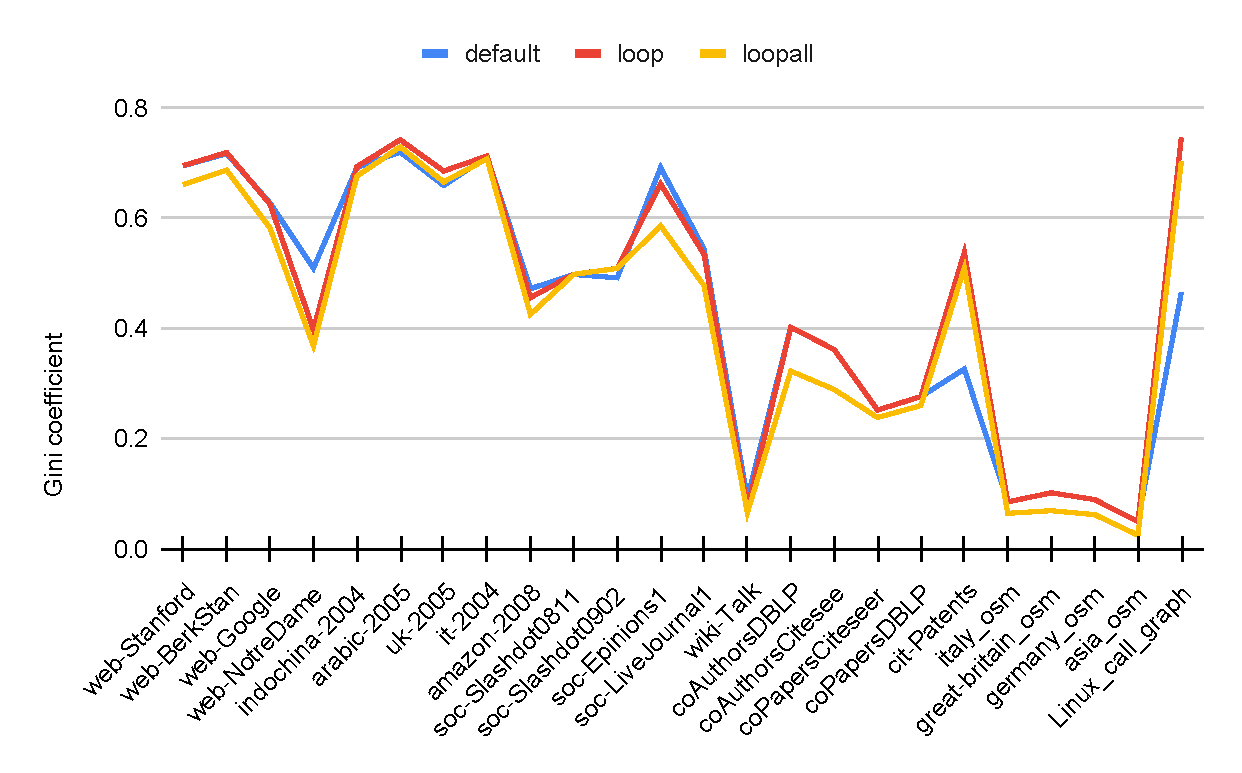
\includegraphics[width=0.68\linewidth]{out/de-gini.pdf}
  } \\[-2ex]
  \caption{Gini coefficient of PageRank values on 24 different graphs, comparing between PageRank values obtained with three different dead-end handling strategies: \textit{teleport from dead-ends} (\textbf{default}), \textit{self-loop dead-ends} (\textbf{loop}), and \textit{self-loop all vertices} (\textbf{loopall}).}
  \label{fig:de-gini}
\end{figure*}

